\documentclass[american,a4paper,12pt]{article}
\usepackage[T1]{fontenc} %for å bruke æøå
\usepackage[utf8]{inputenc}
\usepackage{minted}
\usepackage{graphicx} %for å inkludere grafikk
\usepackage{verbatim} %for å inkludere filer med tegn LaTeX ikke liker
\usepackage[ruled,vlined]{algorithm2e}
\usepackage{algpseudocode} % lager pseudokode til algoritmene
\usepackage{caption}
\usepackage{physics}
\usepackage{multicol}
\usepackage{siunitx}
\usepackage{float}
\usepackage{subcaption}
\usepackage{hyperref}
%\usepackage{biblatex}

\hypersetup{
    colorlinks=true,
    linkcolor=black,
    filecolor=magenta,
    urlcolor=blue,
    citecolor=blue
    %pdftitle={Project 1: Computational Physics - FYS3150},
    %pdfpagemode=FullScreen
}

\renewcommand{\vec}[1]{\mathbf{#1}} %ny definisjon av \vec så det blir bold face i stedet for vector-pil.

\newcommand{\ME}{\ensuremath{M_{\text{Earth}}}} %\ME -> Mass of Earth
\newcommand{\MS}{\ensuremath{M_{\odot}}} %\MS -> Mass of Sun
\newcommand{\ddx}[1]{\frac{\dd #1}{\dd x}} % \ddx{f} = \frac{\dd f}{\dd x}


\captionsetup[table]{skip=10pt}

\title{Building a model of the Solar System using ordinary differential equations to solve the equations of motion}
\author{Fredrik Hoftun \& Mikkel Metzsch Jensen}
\date{\today}
\begin{document}
\maketitle

\begin{abstract}
   In this project we have used different numerical ordinary differential equation solvers to simulate a Solar System model. We were able to successfully simulate stable orbits and affirm laws of nature, like conservation of mechanical energy and total angular momentum. We concluded that the velocity Verlet method is the superior ODE-solver for this particular problem, as it conserves energy and have a smaller global error without any significant expense of run time.\\ We introduced a modified gravitational force, the inverse $\beta$ force, which scaled the exponent for the distance $r^\beta, \beta \in [2,3]$ and saw that it affected the stability of the system greatly.\\ We also looked at how the number of celestial objects simulated in a Newtonian model affected the positional precision of said objects. We found that the precision decreased as the number of objects increased.\\ Finally, we calculated the perihelion precession of Mercury around the Sun for classical forces to $p_{cy,c}=-8\pm 13''$ and general relativistic gravitational forces to $p_{cy,r}=43.5\pm 0.8''$ from which we found a total precession of $P_{cy} = 51.5 \pm 13$. The big uncertainty originates from possible errors in our classical model, but the results still fits with the predicted value of 43".
\end{abstract}
\vfill
\footnotesize{{Link to our GitHub repository: \url{https://github.com/mikkelme/project3_FYS3150}}}
\newpage


\section{Introduction}
The study of the Solar System is a scientific discipline which dates back to the Ancient Era, where mankind observed the nearest planets and stars with the naked eye. As we have gained more insight into this field we have gone through several paradigm shifts regarding our worldview and our small role in the big universe. Some of the biggest shifts came from discoveries like Copernicus' Sun centered system and Newton's theory of gravity, but it is still refined in modern science with the introduction of Einstein's theory of relativity and perhaps also quantum mechanics. In this project we aim to develop a numerical model of the Solar System which makes us able to simulate and predict the movement of several celestial objects. While the analytical solutions are limited to the two-body problem, we can easily compute simulations of a three-body problem or more. Once equipped with a model that describes the force interaction between the celestial objects we can solve the equations of motion as sets of coupled ordinary differential equations (ODE). For this purpose there exists a variety of algorithms. We are going to use the forward Euler method and the velocity Verlet method.\\ 
Starting off we are going to implement a hypothetical solar system consisting of only the Earth orbiting the Sun. We will then run a series of test in order to ensure that our method provide stable and energy conserving orbits. We will also use this opportunity to compare the performance of the two ODE-solver algorithms, and settle on the most effective for the further investigations. Then we will calculate the escape velocity analytically and numerically and introduce a variation of the gravitational force as $F_G = \frac{GmM}{r^{\beta}}$ with $\beta \in [2,3]$ to see how the modified gravitational force affects the system.\\ Afterwards, we will expand the system to include Jupiter with the purpose of testing how it affects the stability of the Earth-Sun system. Later we will include all the other planets and Pluto to our system, resulting in a ten-body-problem. For this section we will use data from NASA's Jet Propulsion Laboratory (JPL) to initialize the celestial objects with positions and velocities with respect to the Solar System center of mass.\\ Finally, we will investigate one of the tests of general relativity, the perihelion precession of Mercury. According to observation the perihelion precession of Mercury disagrees from the predicted Newtonian theory by $\approx 43 ''$ (arcseconds/Julianan century). In general relativity this difference is nonexistent. We will implement a relativistic correctional gravitational force from general relativity to see if we can reproduce this difference and affirm Einstein's theory of general relativity.


\newpage
\section{Method}
\subsection{Setting up the Earth-Sun system}
In the beginning we will limit ourselves to a hypothetical solar system with only the Earth orbiting the Sun. The only force in this problem is the gravitational force $F_G$ acting between the Earth and the Sun. This can be described with Newton's law of gravity as:
\begin{align*}
    F_G = \frac{G\MS\ME}{r^2}
\end{align*}
where $M_{\odot}$ is the mass of the Sun and $M_{Earth}$ is the mass of the Earth. $G$ is the gravitational constant and $r$ is the distance between the Earth and the Sun. Since the mass of the Sun is much larger than that of the Earth we can assume that the Sun is fixed at the origin. By using Newtons second law of motion we arrive at the following differential equation that describe the motion of the Earth:
\begin{align*}
    \vec{a} = \frac{d^2\vec{r}}{dt^2} = \frac{\vec{F_G}}{\ME}, \quad \vec{r} = (x, y, z)
\end{align*}
For the numerical approach we split this into three equations for the Cartesian coordinates x,y and z:
\begin{equation}
    \frac{d^2x}{dt^2} = \frac{F_{G,x}}{\ME}, \qquad 
    \frac{d^2y}{dt^2} = \frac{F_{G,y}}{\ME}, \qquad
    \frac{d^z}{dt^2} = \frac{F_{G,z}}{\ME}
    \label{eq:Earth_ODE}
\end{equation}
where $F_{G,x}$, $F_{G,y}$ and $F_{G,z}$ are the $x$, $y$ and $z$ components of the gravitational force. By using the fact that the Earth's orbit around the Sun is almost circular we can assume the following relation from the centripetal force:
\begin{align*}
    \frac{\ME v^2}{r} = \frac{G\MS\ME}{r^2}
\end{align*}
where $v$ is the tangential velocity. The latter equation can be solved to show that:
\begin{align*}
    v = \sqrt{\frac{G\MS}{r}} 
\end{align*}
We introduce "Astronomical units" where we define mass as mass relative to the solar mass $\MS$, time as Julianan years $1 \text{yr} = 365.25\ \text{days},1\ \text{day} = 86400\ \text{s} $, and distance as one astronomical unit $1 \text{AU} = 149\ 597\ 870\ 700$m (approximately the mean distance between the Sun and Earth). By using the follow unit conversion: 
\begin{align*}
     &[m] = \frac{1}{149\ 597\ 870\ 700} \ \text{AU}&  &[s] = \frac{1}{365.25 \cdot 86400} \text{yr}&   &[kg] = 1.98847\cdot 10^{-30} \MS&
\end{align*}
we can recalculate the value of $G$ as:
\begin{align*}
    G = 6.67408 \cdot 10^{-11} \frac{m^3}{s^2 kg} = 39.477 \ \frac{AU^3}{yr^2\MS}  \approx 4 \pi^2 \ \frac{AU^3}{yr^2\MS}
\end{align*}
We then see that a circular orbit for the Earth at $r = 1$ AU must have a tangential velocity of $v = 2 \pi\ \text{AU/yr}$.

\newpage
\subsubsection{Algorithms for solving ordinary differential equations}
In order to solve the ordinary differential equations (ODE) displayed in the previous section (see equation \ref{eq:Earth_ODE}) we will use both the the Forward Euler and the Velocity Verlet method. The Euler method is the simplest possible ODE-solver and can be derived from the Taylor expansion of a function f around a value $t_0+dt$:
\begin{align*}
    f(t_0 + dt) = f(t_0) + dtf'(t_0) + \mathcal{O}(dt^2)
\end{align*}
where f is a differentiable function of t and dt is a small timestep. This approximates the evolution of f as t is increased by dt.  We can substitute in the the equations of motions from (\ref{eq:Earth_ODE}) for a solution to our problem. For the x-component as an example we get:
\begin{align*}
    a_x = \frac{d^2x}{dt^2} &= \frac{F_{G,x}(\vec{r}(t))}{\ME} \\
    v_x(t+dt) &= v_x(t) + a_x(t)dt\\
    x(t+dt) &= x(t) + v_x(t)dt
\end{align*}
This can easily be discretized as:
\begin{align*}
    a_{x,i} &= \frac{F_{x,i}}{\ME} \\
    v_{x,i+1} &= v_{x,i} + a_{x,i}dt\\
    x_{i+1} &= x_i + v_i dt
\end{align*}
The local error done in each step is $\mathcal{O}(dt^2)$ which mean that the global error for a simulation of $T$ years with $N = T/dt$ timesteps is $\mathcal{O}(N)$. The number of FLOPs for the Euler method is $N(5 + F(F_G))$ where $F(F_G)$ is the number of FLOPs needed to calculate the gravitational force $F_G$. For the Earth-Sun system we have $F(F_G) = 4$, two for the numerator, one for the denominator and one for the fraction itself. This however can be reduced to $F(F_G) = 3$ by pre-calculating the denominator (as it is constant). However, in reality the gravitational force is three dimensional, so the time needed to calculate should go like $\approx 3N$. This can be mitigated by vectorizing the gravitational force and algorithms:
\begin{align*}
    \vec{F_G} = -\frac{G \MS \ME}{r^2} \hat{\vec{r}} = -\frac{G \MS \ME}{r^3}\vec{r}
\end{align*}
where $\hat{\vec{r}} = \frac{\vec{r_S-r_E}}{|\vec{r_S-r_E}|}$ is the positional unit vector. The time then gets reduced back to $\approx N$ as all three dimensions are calculated simultaneously.

\newpage
It is a well known fact that the Euler method is quite inefficient for bigger calculations as it needs a very small step length $dt$ to get satisfactory results in most cases. The Euler method is not a symplectic ODE-solver, meaning that it will not conserve energy very well. The velocity Verlet method on the other hand is a symplectic ODE-solver specifically designed for solving the equations of motion\cite{verlet}. It can be derived by Taylor expanding $x(t + dt)$:
\begin{align*}
    x(t+dt) &= x(t) + \frac{v_x(t)}{1!}dt + \frac{a_x(t)}{2!}dt^2 + O(dt^3)\\
    v_x(t+dt) &= v_x(t) + \frac{a_x(t)}{1!}dt  +  \frac{a_x'(t)}{2!}dt^2 + O(dt^3)\\
    a_x(t+dt) &= a_x(t) + \frac{a_x'(t)}{1!}dt + O(h^2) \overset{\approx}{\to} a_x'(t)dt = a_x(t+dt) - a_x(t)\\
    v_x(t+dt) &= v_x(t) + \frac{a_x(t+dt) + a_x(t)}{2}dt + O(dt^3)
\end{align*}
which can be easily discretized as
\begin{align*}
     a_{x,i} &= \frac{F_{x,i}}{\ME} \\
    x_{i+1} &= x_i + v_{x,i} dt + a_{x,i} \frac{dt^2}{2}\\
    v_{x,i+1} &= v_{x,i} + \frac{a_{x,i} + a_{x,i+1}}{2}dt
\end{align*}
The global error of this method goes like $\mathcal{O}(dt^2)$ while the number of FLOPs required: $N(12 + 2 F(F_G))$ is still proportional to N like the Euler method. 

\subsubsection{Conservation of angular momentum}
Kepler's second law of planetary motion states: "A line connecting the Sun and the planet sweeps out equal areas in an equal time interval"\cite{kepler}. Mathematically we can express this area sweep as:
\begin{align*}
    \frac{\dd A}{\dd t} = \frac{r^2 \dd \theta}{2\ \dd t} = \frac{L}{2m}
\end{align*}
where $L$ is the angular momentum. The change in the angular momentum with respect to time defines the torque on the system $\tau = \frac{\dd L}{\dd t}$, which can also be described as $\tau = r \cross F$. Since gravity is the only force acting in the Earth-Sun system and it is parallel to the position vector $r$ we get:
\begin{align*}
    \tau = r \cross F = \frac{\dd L}{\dd t} = 0
\end{align*}
From this we can tell that the angular momentum must remain constant in the Earth-Sun system.
The angular momentum of a a two-body gravity must therefore always be conserved, since the positional vector and force vector are always parallel. In a simulation with three or more bodies the individual angular momenta are not conserved, as we get cross-products between forces and positional vectors that are not parallel. However the total angular momentum of the system is conserved because of the rotational symmetry of the gravitational force. This means that the total angular momentum is conserved in a system consisting of the Sun, all the planets and Pluto or other similar systems.

\newpage
\subsubsection{Testing forms of the force}
Till now we have assumed that gravity is an inverse square force:
\begin{align*}
    F_G = \frac{G\MS\ME}{r^2}
\end{align*}
but we will investigate the consequences of having an "inverse $\beta$" force:
\begin{align*}
    F_G = \frac{G\MS\ME}{r^{\beta}}
\end{align*}
with $\beta \in [2,3]$. We will run simulations on the Earth-Sun system using the velocity Verlet method for different values of $\beta$ and test whether or not the system is stable in terms of position and energy conservation. 


\subsubsection{Escape velocity}
The escape velocity is defined as the velocity where the kinetic and the potential energy are equal:
\begin{align*}
    \frac{1}{2} \ME v^2 &= \frac{G \MS \ME}{r}
\end{align*}
and we find the esacpe velocity $v_{esc}$ as: 
\begin{align*}
    v_{esc} &= \sqrt{2 G \MS /r}
\end{align*}
If $r = 1 AU$ we get:
\begin{align*}
    v_{esc} &= \sqrt{2 \cdot 4 \pi^2} \approx 8.857 AU/yr = 42.14 km/s
\end{align*}
In order to the test our implementation of the Solar System model, we will approximate this value numerically. This is done by setting up a simplified system where the earth is initialized with $\vec{r}$ = (1 AU, 0, 0) and velocity $\vec{v}$ = ($v_{test}$, 0, 0). If the test speed $v_{test}$ is lower than the escape velocity it should eventually change direction and come back to the Sun. We therefore set up a algorithm that checks whether the velocity x-component change sign during the simulation time. We then increase $v_{test}$ until we no longer see the Earth turning around. We use a simulation time of $T = 1000$ yr and $dt = 0.01$ yr. 

\subsection{Expanding the Earth-Sun system}
We now want to expand our Earth-Sun system to include Jupiter. The simplest way to do this is using the vector formulation of Newton's law of gravity:
\begin{align*}
    F_G &= -G \frac{M m}{|\vec{r}|^3}\vec{r}
\end{align*}
where $M$ and $m$ are the masses of the two objects, $\vec{r}$ is the positional vector between them and $|\vec{r}|$ is the length of the positional vector (the distance between the objects).
\newpage
We know that the gravitational force on Earth is the sum of the gravitational forces from the Sun and Jupiter
\begin{align*}
    F &= F_S + F_J\\
    &= -G \frac{\MS \ME}{|\vec{r_S}-\vec{r_E}|^3}(\vec{r_S}-\vec{r_E}) -G \frac{M_{Jupiter} \ME}{|\vec{r_J}-\vec{r_E}|^3}(\vec{r_J}-\vec{r_E})
\end{align*}
where $\vec{r_S}-\vec{r_E}$ is the positional vector between the Sun and Earth, $M_{Jupiter}$ is the mass of Jupiter, and $\vec{r_J}-\vec{r_E}$ is the positional vector between Jupiter and Earth. This can easily be generalized as:
\begin{equation}
    F_{ij} = -\sum_{j=1,j\neq i}^n G \frac{M_i M_j}{|\vec{r_j} - \vec{r_i}|^3}(\vec{r_j}-\vec{r_i})
    \label{eq:Fij}    
\end{equation}

where $M_i$ is the mass of the planet receiving the forces from planets with mass $M_j$, $n$ is the number of planets, $\vec{r_j} - \vec{r_i}$ are the positional vectors from the planets $j$ to planet $i$ and $|\vec{r_j} - \vec{r_i}|$ are the lengths of the positional vectors, the distances between the planets $j$ and planet $i$. From this we can easily implement as many celestial objects as we desire. 

\subsection{Object orientation}
In order to generalize the code for a many-body problem using equation \ref{eq:Fij} we modify it using object orientation. The structure of the code can be briefly outlined by the following summary of the classes we have implemented in $\verb!C++!$ (see our GitHub repository \cite{project3} for more details):
\begin{itemize}
    \item CelestialBody: Contains a constructor for the celestial object with all the associated values: position, velocity, mass, force and energy. 
    \item SolarSystem: Contains all the CelestialBody instances added and functions which manage calculation of force and energy and writing to file.
    \item Solver: Contains the algorithms for solving the ODE's.
    \item Force: Contains needed force formulas: Newtons gravitational force, inverse beta and General relativistic correction to Newtons gravitational force. The calculation of energy is placed here as well as the potential energy is related to the force. 
\end{itemize}
The way we deal with the many problem is to run a double for-loop in order to calculate the force between every celestial body. This loop is placed in the SolarSystem class and are called by the solvers for each timestep.
\newpage
It can look something like this: \\
\begin{algorithm}[H]
\SetAlgoLined
List of bodies = bodies;\
Number of bodies = N\;
\For{\forcond{(i = 0; i < N; i++)}}
    {body1 = bodies[i]\;
    \For{\forcond{(j = i+1; j < N; j++)}}
        {body2 = bodies[j]\;
        //Call force class for calculation of force and energy\;
        Force(body1, body2)\;
        Force(body2, body1)\;
    }
}
 \caption{Calculation of force and energy for a many body system.}
\end{algorithm}
The calling of the force class will then link to the chosen force model and calculate the force and energy on body1 with respect to body2 and likewise for body2 with respect to body1. See Appendix for details about the calculation of energy. The values are added to the existing one (not replaced) so we can gather the contribution from every body. Therefore we also have to reset this between every time-step. 

\subsection{Mercury perihelion precession}
As a test of general relativity we want to reproduce the perihelion precession of Mercury around the Sun. The observed precession deviates with 43'' per century from the predictions made from the Newtonian gravitational force and all other classical effects. By using a general relativistic correction the force becomes:
\begin{align}
    F_G = \frac{G\MS M_{\text{Mercury}}}{r^2}(1 + \frac{3l^2}{r^2c^2})
    \label{eq:GR_gravity}
\end{align}
where $M_{\text{Mercury}}$ is the mass of Mercury, $r$ is the distance between Mercury and the Sun, $l = |\vec{r} \times \vec{v}|$, is the magnitude of Mercury's orbital angular momentum per unit mass, and $c$ is the speed of light in vacuum. We are going to run a simulation of Mercury's orbit starting from the perihelion (position closest to the sun) using the initial values:
\begin{align*}
    \vec{r} = (0.3075 \ \text{AU}, 0, 0), \qquad \vec{v} = (0, 12.44 \ \text{AU/yr}, 0)
\end{align*}
with the Sun fixed at the origin. We will then run the simulation for a 100 years. From the Python module SciPy we import a function called scipy.signal.argrelextrema\cite{argrelextrema} in order to find local minema on the radial distance data. This makes us able to determine the x,y position for every time Mercury passes the perihelion position. We can then calculate the angle between the x-axis and perihelion using:
\begin{align*}
    \tan{\theta_p} = \frac{y_p}{x_p}
\end{align*}
We do this with and without the general relativistic correction and compute the difference. If the time-interval $dt$ is sufficiently small we expect the value from the classical case to be almost zero because we have no disturbing planets in this simulation. We expect the value in the relativistic case to approach the observed difference of 43''.

\newpage
\section{Results}
\subsection{Earth-Sun System}
\subsubsection{Comparing solvers}
In the initial setup we have the Sun fixed at the origin and Earth at position $\vec{r}$ = (1 AU, 0, 0) and velocity $\vec{v}$ = (0, $2\pi$ AU/yr, 0) in order to get a circular orbit in the x,y-plane. We then simulated the motion of the Earth for $T$ = 10 yr with $dt = 0.001$ yr for both solvers shown in figure \ref{fig:ES_initial_run}. The results are produced with the executables "EarthSun\_Euler.exe" and "EarthSun\_Verlet.exe" \cite{testfiles}.
\begin{figure}[H]
  \centering
  \begin{minipage}[b]{0.49\textwidth}
    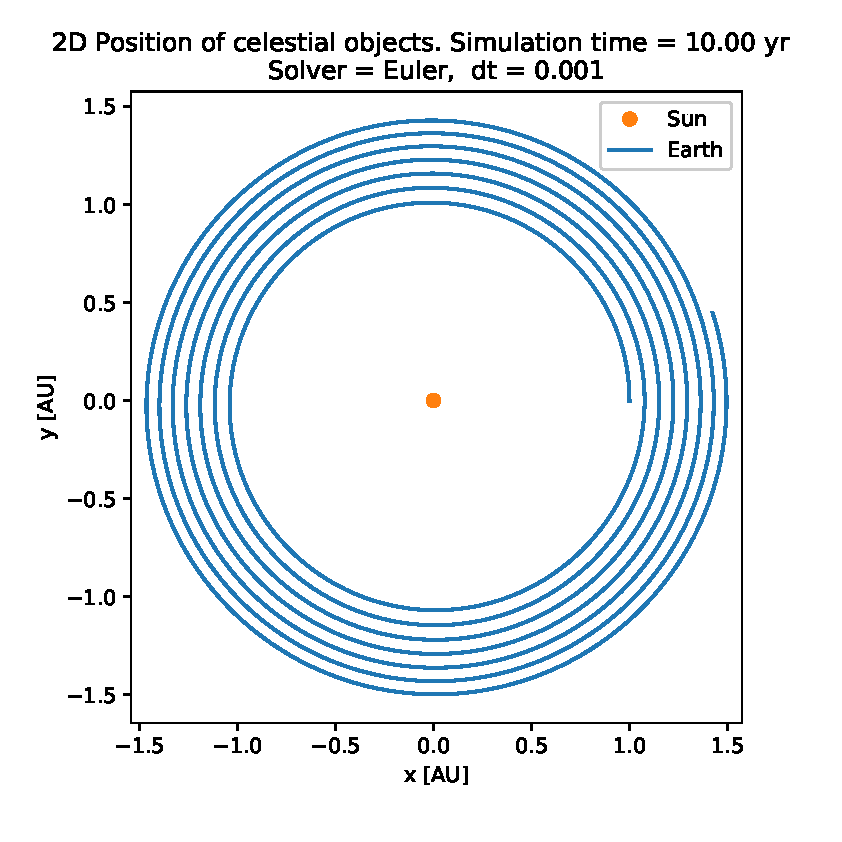
\includegraphics[width=\textwidth]{figures/Earth_Sun_10yr_Stable_Euler.eps}
  \end{minipage}
  \hfill
  \begin{minipage}[b]{0.49\textwidth}
    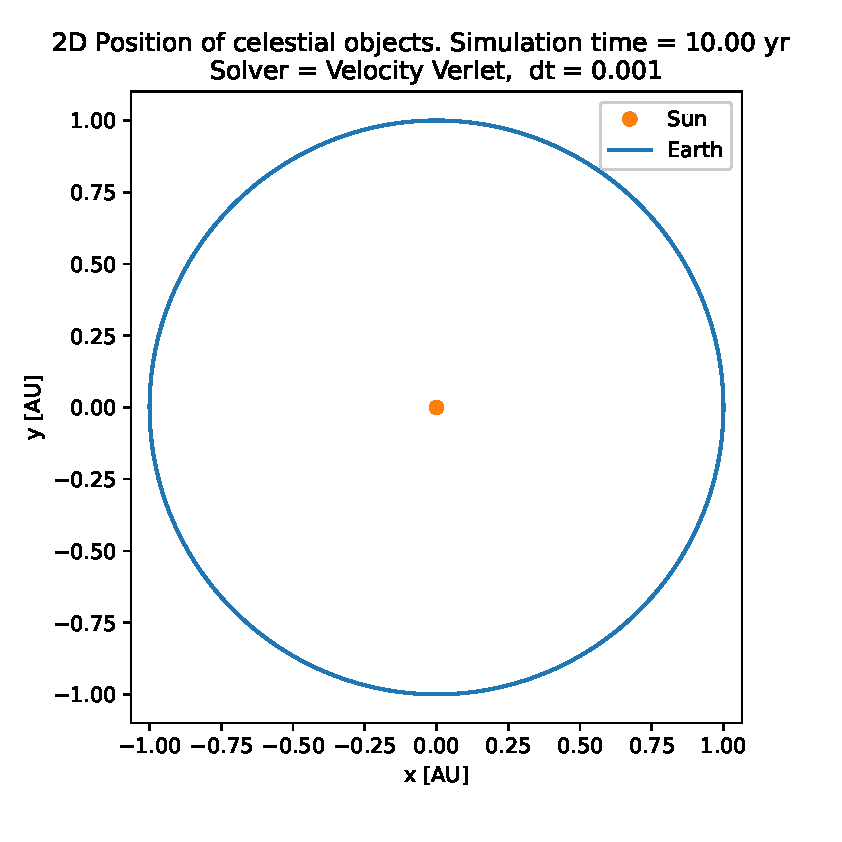
\includegraphics[width=\textwidth]{figures/Earth_Sun_10yr_Stable_Verlet.eps}
  \end{minipage}
  \caption{Simulation of Earth-Sun system for $T = 10$ yr, $dt = 0.001$ 1/yr with the Sun fixied at the origin. Shows better stability for the Velocity Verlet salgorithm than the Euler algorithm}
  \label{fig:ES_initial_run}
\end{figure}
From this test we see quite a big difference in the stability of the two solutions. We then ran the same 10 year simulation for both solvers for $dt \in [0.1, 10^{-5}]$. Since we retain the initial values for a circular orbit we expect the Earth to return to its original position after any whole number of years. Therefore we can calculate the positional error as the difference between the first and last positions. In addition we calculate the difference in the total mechanical energy as this should also be conserved. The results are produced with the executables "EarthSun\_Euler.exe" and "EarthSun\_Verlet.exe" and shown in figure \ref{fig:ES_error}. 
\begin{figure}[H]
    \centering
    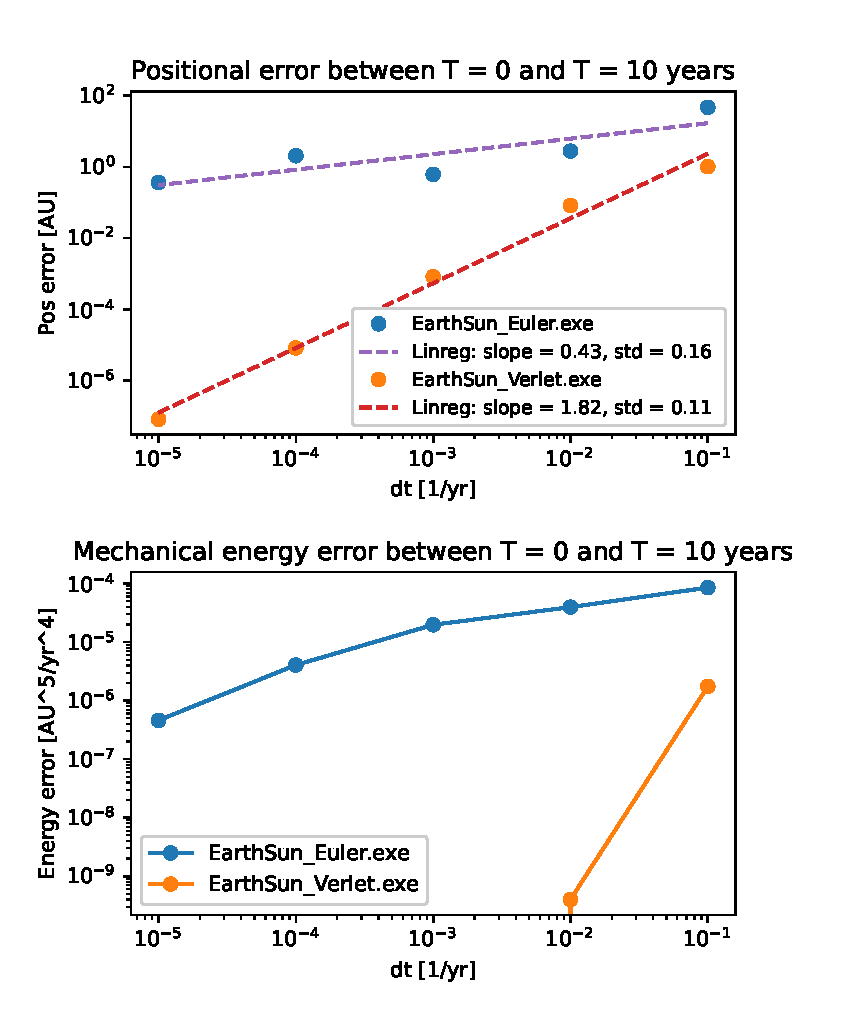
\includegraphics[width =0.9\textwidth]{figures/Earth_Sun_10yr_error.eps}
    \caption{Plot of the relation between positional error and total mechanical error with respect to time.step $dt$. The simulation is initialized to be circular and the Sun is fixed at the origin. We see clear differences in the performance of the two algorithms.}
    \label{fig:ES_error}
\end{figure}
We also ran a timing of the two algorithms while simulation the circular Earth-Sun system. For this purpose we disabled the writing to file and did not use any compiler flags for speed up. The result are produced with the executables "Euler\_timing.exe" and "Verlet\_timing.exe" and showed in figure \ref{fig:ES_timing}.
\begin{figure}[H]
    \centering
    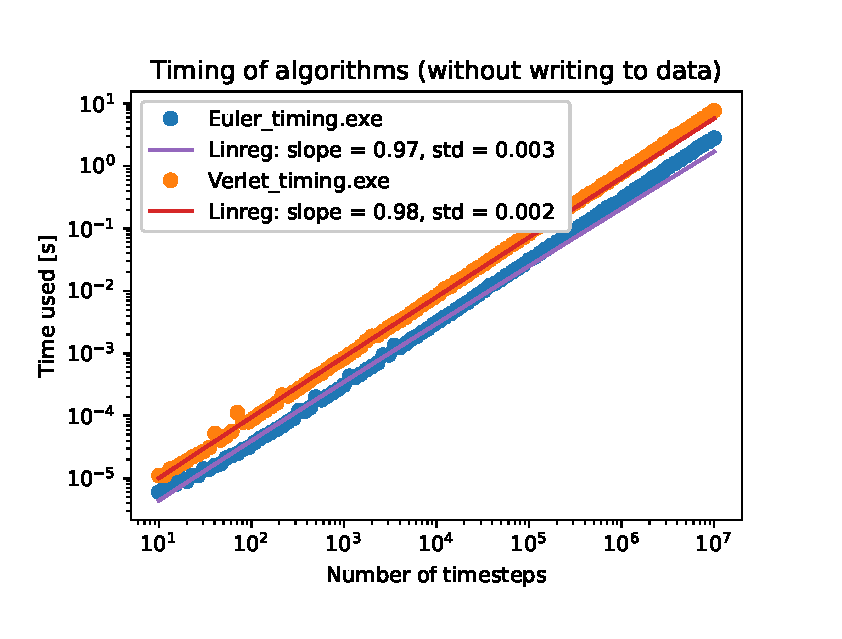
\includegraphics[width = \textwidth]{figures/EarthSun_timing.eps}
    \caption{Timing of the two algorithms for a 10 year simulation of the circular Earth-Sun system with dt = 0.001. Writing to file is disabled and no compile flags used.}
    \label{fig:ES_timing}
\end{figure}
\subsubsection{Testing the inverse $\beta$ force}
We now introduce the inverse beta force to the Earth-Sun system. We keep the sun fixed but now we initialize an elliptical orbit with Earth at position $\vec{r}$ = (1 AU, 0, 0) and velocity $\vec{v}$ = (0, 5 AU/yr, 0). First we simulate the position over 10 years for 16 evenly spread out values of $\beta \in [2,3]$ (see figure \ref{fig:IB_pos}). The following results in this section are all produced with the executable "EarthSun\_InverseBeta\_ellipse.exe".
\begin{figure}[H]
    \centering
    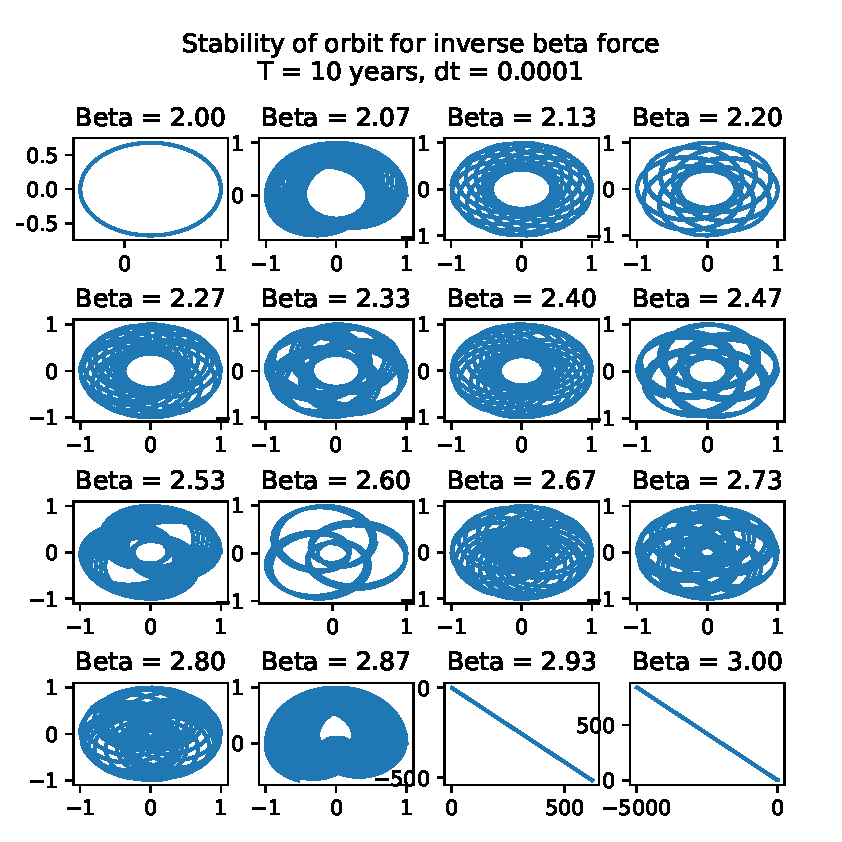
\includegraphics[width = \textwidth]{figures/EarthSun_InverseBeta_pos.eps}
    \caption{Positional display of the elliptical orbit of the Earth-Sun system for the inverse beta force for different values of $\beta$. The axis show x,y position in AU, but this is removed to make is easier to see the results.}
    \label{fig:IB_pos}
\end{figure}
We then looked at the energy difference between the first and last time-step of the elliptical orbit with inverse beta force. We reduced the run time to just a half year but increased the number of points for $\beta$ to 1001. The result are showed in figure \ref{fig:IB_energy}.
\begin{figure}[H]
    \centering
    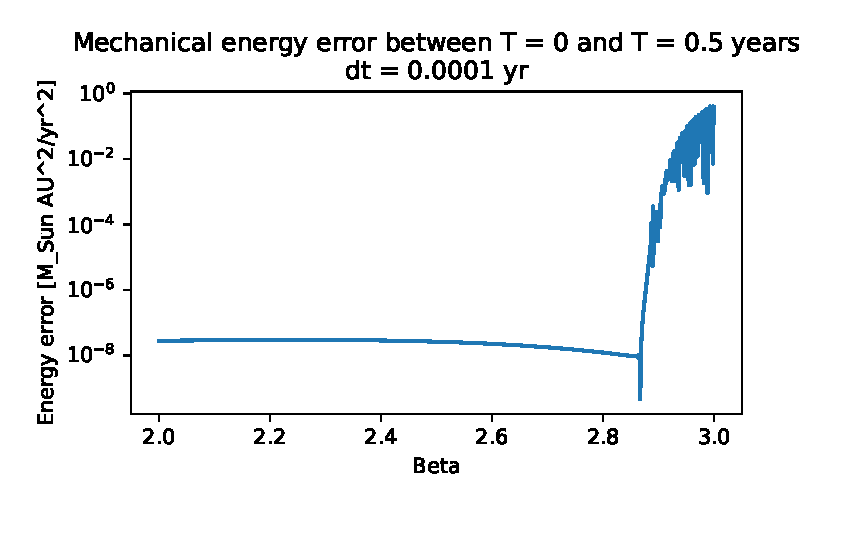
\includegraphics[width = \textwidth]{figures/EarthSun_InverseBeta_energy.eps}
    \caption{Energy error bewteen T = 0 and T = 0.5 years  for the elliptical Earth-Sun system with inverse beta force.}
    \label{fig:IB_energy}
\end{figure}
Since the energy error seem to increase around $\beta = [2.87, 2.89]$ we took a closer look at the radial distance between the Earth and the Sun in that interval. This is showed in figure \ref{fig:IB_radial}.

\begin{figure}[H]
    \centering
    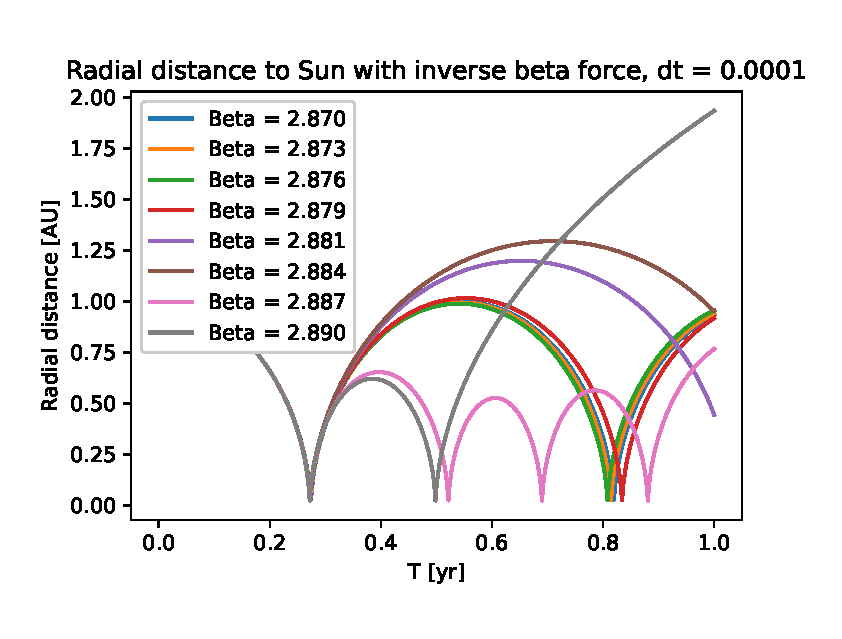
\includegraphics[width = \textwidth]{figures/EarthSun_InverseBeta_radial.eps}
    \caption{The radial distance between the Earth and the Sun for the elliptical Earth-Sun system with inverse beta force.}
    \label{fig:IB_radial}
\end{figure}

Note that the precise tipping point for the stability loss seemed to be dependent on the choice of $dt$. While the tipping point shown here for $dt = 0.0001$ is in the interval $\beta \in [2.887, 2.890]$ this was in the interval $\beta \in [2.876, 2.879]$ for $dt = 0.001$. On the other hand the angular momentum was constant for any choice of $beta \in [2,3]$ (se figure \ref{fig:IB_L}).

\begin{figure}[H]
    \centering
    \includegraphics[width = \textwidth]{figures/EarthSun_InverseBeta_L.eps}
    \caption{The angular momentum of the Earth with respect to the Sun fixed at the origin for the elliptical Earth-Sun system with the inverse beta force.}
    \label{fig:IB_L}
\end{figure}


\subsubsection{Escape velocity}
With our knowledge of the analytical escape velocity we ran a test with starting velocity close to the analytical answer and increased the velocity by 0.0001 AU/yr each time the speed was found to be insufficient to satisfy the 1000 years escape criteria. From this we got: 
\begin{align*}
    &v_{escape} = 8.8785 \pm 0.0001& &\text{relative error} = 0.0818 \%& 
\end{align*}

\subsection{Earth-Sun-Jupiter system}
Here we have introduced Jupiter to the elliptical Earth-Sun system. We got the initial conditions for Earth and Jupiter from NASA JPL's HORIZON web-interface \cite{JPL}. The time of initial conditions were: date, time of day = October 23rd 2020, 00:00:00.0000. The Sun was fixed at the origin so we could compare the stability to the Earth-Sun system. For further investigation we decided to create two additional systems, were the mass of Jupiter were 10- or 1000 times its original mass. The results from the Earth-Sun system and Earth-Sun-Jupiter systems are shown side by side on figures \ref{fig:ES_eliptical}, \ref{fig:ESJ_fixed}, \ref{fig:Jupiter10} and \ref{fig:Jupiter1000} below:
\begin{figure}[H]
  \centering
  \begin{minipage}[b]{0.49\textwidth}
    \includegraphics[width=\textwidth]{figures/Earth.png}
    \caption{Earth-Sun system.}
    \label{fig:ES_eliptical}
  \end{minipage}
  \hfill
  \begin{minipage}[b]{0.49\textwidth}
    \includegraphics[width=\textwidth]{figures/Jupiter.png}
    \caption{Earth-Sun-Jupiter system.}
    \label{fig:ESJ_fixed}
  \end{minipage}
\end{figure}
We then tried increasing Jupiter's mass by a factor 10 and 100 respectively (see figure \ref{fig:Jupiter10} and \ref{fig:Jupiter1000}.
\begin{figure}[H]
  \centering
  \begin{minipage}[b]{0.49\textwidth}
    \includegraphics[width=\textwidth]{figures/Jupiter10.png}
    \caption{Earth-Sun-Jupiter system, where Jupiter's mass is 10 times it's original mass.}
    \label{fig:Jupiter10}
  \end{minipage}
  \hfill
  \begin{minipage}[b]{0.49\textwidth}
    \includegraphics[width=\textwidth]{figures/Jupiter1000.png}
    \caption{Earth-Sun-Jupiter system, where Jupiter's mass is 1000 times it's original mass.}
    \label{fig:Jupiter1000}
  \end{minipage}
\end{figure}

\newpage
The positional and mechanical energy stability of the systems:
\begin{figure}[H]
    \centering
    \includegraphics[width=0.85\textwidth]{figures/Earth_Jupiter_stability.png}
    \caption{Positional and energy stability of the different systems.}
    \label{fig:ESJ_stability}
\end{figure}
We can see that all the systems, except for the system where Jupiter is 1000 times its original mass, are relatively equal by looking at the slope-values for the linear fit on the positional error or by looking at the data-points which nearly overlap. However, the positional error is quite large in itself at $\approx 10^{-1/2}$, still nothing compared to the 1000 mass Jupiter system with errors $\approx 10^{1,2}$. We also see that the mechanical energy error of the system gets worse as Jupiter's mass increases. These results of the Earth-Sun-Jupiter system were computed with the executables "Earth.exe", "Jupiter.exe", "Jupiter10.exe" and "Jupiter1000.exe". The positional plots had a time-step $dt = 0.001$ yr, number of steps $10000$ making the total time $Time = 10$ yr.

\newpage
\subsection{All planets system}
\subsubsection{Earth-Sun-Jupiter system, Sun not fixed}
\label{sec:Sun_not_fixed}
We made a similar simulation where the Sun was not fixed at the origin, but had initial position from JPLs HORIZON. We set the initial velocity of the Sun equal to the sum of the Earth's and Jupiter's momentum divided by its mass to prevent the origin from drifting. We got the following 2D positional plots showed in figure \ref{fig:ESJ_unfixed} and \ref{fig:ESJ_Sun}.
\begin{figure}[H]
  \centering
  \begin{minipage}[b]{0.49\textwidth}
    \includegraphics[width=\textwidth]{figures/ESJ.png}
    \caption{Earth-Sun-Jupiter system, where the Sun's position is not fixed at the origin.}
    \label{fig:ESJ_unfixed}
  \end{minipage}
  \hfill
  \begin{minipage}[b]{0.49\textwidth}
    \includegraphics[width=\textwidth]{figures/ESJ_Sun_drift.png}
    \caption{Close-up of the not fixed Earth-Sun-Jupiter system, showing a stable Sun orbit.}
    \label{fig:ESJ_Sun}
  \end{minipage}
\end{figure}

\newpage
\subsubsection{All planets system}
Finally we simulated the All planets system consisting of the Sun and all the planets, including Pluto. The position of the sun and initial conditions of the planets and Pluto were taken from JPLs HORIZON, while the Sun's initial velocity was set equal to the sum of all the momenta divided by its mass. The 2D positional plots from this simulaion are shown in figure \ref{fig:All_planets} and \ref{fig:All_planets_Sun}: 
\begin{figure}[H]
  \centering
  \begin{minipage}[b]{0.49\textwidth}
    \includegraphics[width=\textwidth]{figures/All_planets.png}
    \caption{All planets system.\\The Sun's position is not fixed at\\the origin.}
    \label{fig:All_planets}
  \end{minipage}
  \hfill
  \begin{minipage}[b]{0.49\textwidth}
    \includegraphics[width=\textwidth]{figures/All_planets_Sun_drift.png}
    \caption{Close-up of the All planets system, showing an unstable Sun orbit.}
    \label{fig:All_planets_Sun}
  \end{minipage}
\end{figure}

\newpage
The positional and mechanical energy stability of the systems are shown in figure \ref{fig:All_planets_stability}
\begin{figure}[H]
    \centering
    \includegraphics[width=\textwidth]{figures/All_planets_stability.png}
    \caption{Positional stability of the different systems.}
    \label{fig:All_planets_stability}
\end{figure}
We can see that the positional error does not decrease much as $dt$ decreases, and that the error in itself is quite large at $\approx 10^{-1}$m. The mechanical energy of the system remains almost constant as a function of $dt$ and is more precise compared to the position. These results of the Earth-Sun-Jupiter system and the All planets system were computed with the executables "Earth\_Sun\_Jupiter.exe" and "All\_planets.exe". The positional plots had a time-step $dt = 0.001$ yr, number of steps $100000$ making the total time $T = 100$ yr.

\newpage
\subsection{Mercury perihelion precession}
We ran the Mercury-Sun simulation for for 100 years with dt = 1e-6 and the Sun fixed at the origin. The result is shown on figure \ref{fig:preccession_GR} and is produced with the executable "MercurySun\_precession\_correction.exe".
\begin{figure}[H]
    \centering
    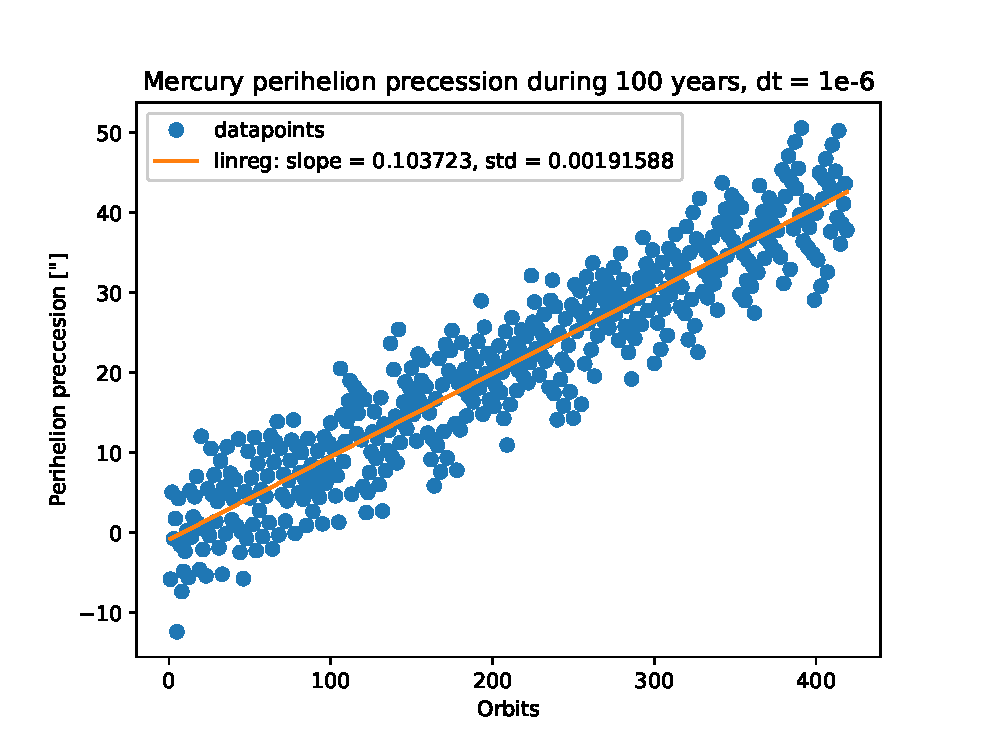
\includegraphics[width = \textwidth]{figures/Mercury_precession.eps}
    \caption{Angle between perihelion and x-axis (starting point) for each orbit of the Mercury-Sun system with the corrected gravitational force during a 100 years period with 419 complete orbits. We see that the angle slowly increases.}
    \label{fig:preccession_GR}
\end{figure}
From our results we get that the perihelion precession per orbit is $p_{\text{orbits}} = 0.104 \pm 0.002 \ "/\text{orbit}$. This were fitted over 419 complete orbits during the exact time 99.90366 years. We can calculate the estimated precession pr. century (cy) as:
\begin{align*}
    p_{cy} = p_{\text{orbit}} \cdot \frac{419 \ \text{orbits}}{99.90366 \ \text{yr}}100 \ \text{yr} = 43.5 \pm 0.8 \ "
\end{align*}
The same simulation with the standard Newtonian gravitational force produced with "MercurySun\_precession\_newton.exe" yielded the results shown on figure \ref{fig:precession_Newton}.
\begin{figure}[H]
    \centering
    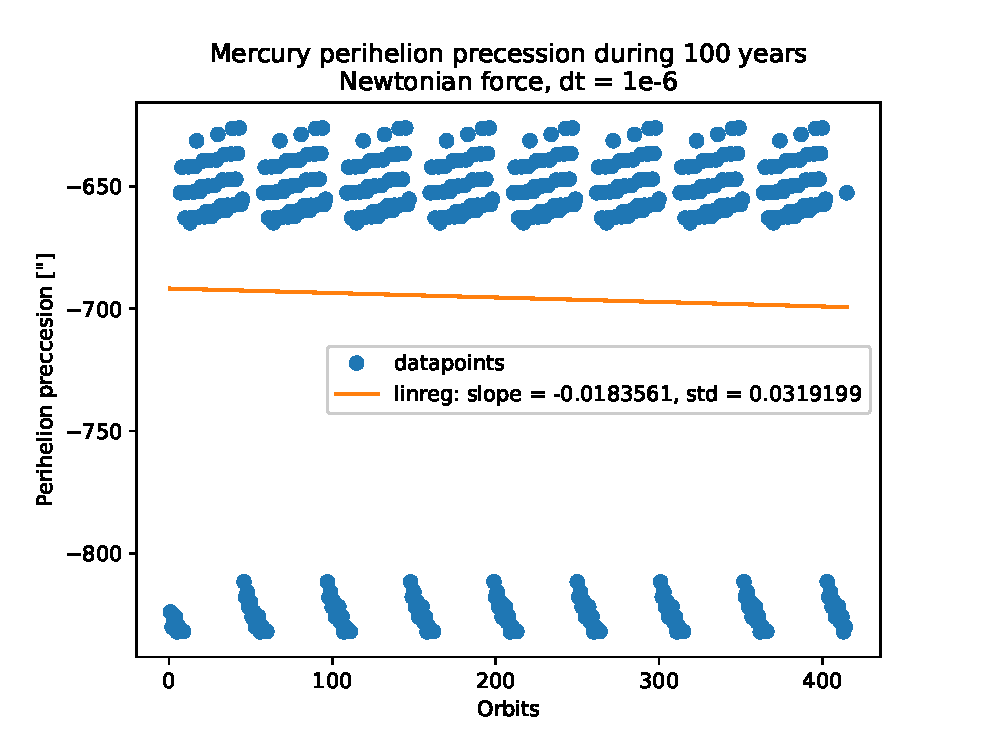
\includegraphics[width = \textwidth]{figures/Mercury_precession_newton.eps}
    \caption{Mercury precession with identical conditions as showed in figure \ref{fig:preccession_GR} expect that we used the standard Newtonian force in this simulation.}
    \label{fig:precession_Newton}
\end{figure}
The results from the simulation with the Newtonian force turned out to be worse than expected, but we did not have time to run double check with a new executable. The algorithm for detecting the local minema only found 415 orbits, and thus we get:
\begin{align*}
    p_{cy} = -8 \pm 13 \ " 
\end{align*}
If we use this result the difference in precession becomes:
\begin{align*}
    \Delta P_{cy} = 51.5 \pm 13
\end{align*}
\newpage
\section{Discussion}
\subsection{Earth-Sun system}
We see that we are able to produce stable orbits with conservation of mechanical energy and angular momentum if the step-length $dt$ is sufficiently small. Conservation of energy was expected since gravity is a conservative force, and the angular momentum should be conserved as there is no torque on the system. We have seen this numerically in figures \ref{fig:ES_error} and \ref{fig:IB_L}. As expected we also found that the errors in position (with respect to the expected value from a circular orbit) and the mechanical energy decreases as the step length $dt$ decreases. This is of course supported by the idea that a smaller step length will grant more precise calculations of the motion of the celestial objects, which will deviate less and less from the analytical solution.
\subsubsection{Comparing solvers}
From figure \ref{fig:ES_error} and \ref{fig:ES_timing} we generally see that the velocity Verlet is superior in numerical stability while using about the same amount of time. From the results we found that the error and time usage of the two algorithms behaves as shown in table \ref{tab:solver_comparison}.
\begin{table}[H]
  \begin{center}
  \caption{Numerical performance of the Euler and Velocity Verlet method as function of step length $dt$ and total number of time steps $N$}
  \label{tab:solver_comparison}
  \begin{tabular}{|c|c|c|} \hline
  \textbf{Sovler} & \textbf{Global error} & \textbf{Time} \\ \hline
  Euler & $\mathcal{O}(dt^{0.4})$ & $\mathcal{O}(N^{0.97})$  \\
  \hline
  Velocity Verlet & $\mathcal{O}(dt^{1.8})$ &  $\mathcal{O}(N^{0.98})$ \\
  \hline
  \end{tabular}
  \end{center}
\end{table}
From a theoretical standpoint we expected the global error to be $\mathcal{O}(dt^{1})$ for the Euler method and $\mathcal{O}(dt^{2})$ for the Verlet method respectively. So in practice the Euler turned out to be even worse while the Velocity Verlet was just slightly worse than the expected value. This can perhaps be explained by the fact that the Velocity Verlet is a symplectic ODE as opposed to the Euler method. This characteristic is clearly showcased in figure \ref{fig:ES_error} where we see that the energy error decreases drastically towards zero in the velocity Verlet for decreasing $dt$ while the Euler method still carried a sizable energy error at dt = $10^{-5}$. 

\subsubsection{Inverse $\beta$ force}
From the simulations with the Inverse $\beta$ force we clearly saw that a change in $\beta$ affected the stability of the system. This is very well showcased in figure \ref{fig:IB_pos} where we see various different orbits with elliptical motion. As we approached $\beta$ = 3 the system became unstable and the Earth was thrown out of orbit. We tried to narrow down this limit by looking at the energy conservation and the radial distance. With the use of dt = 0.0001 we found the instability limit to be in the interval $\beta \in [2.887, 2.890]$. But this limit was found to be dependent of $dt$, such that a smaller $dt$ pushed the instability point further towards 3. When looking at the radial distance we see that the orbit became very elliptical, and the small distance to the Sun (high force) and big velocities might lead to numerical errors.\newpage This also explains the sudden loss of mechanical energy and the fact that the Earth was able to escape the gravitational pull from the Sun, as shown in figure \ref{fig:IB_pos} for $\beta = 2.93$ and 3.00. Therefore we can't say whether the instability limit is connected to the nature of the force or just pure numerical errors. On the other hand we can tell that the amount nature deviates from a perfect inverse-square law is extremely small, as only values of $\beta \approx 2.00$ were similar to Earth's orbit. Regarding the observation of constant angular momentum, we know that this comes from the fact that the torque on the system is always $0$ for a two-body system since the force unit-vector is the same regardless of $\beta$.

\subsubsection{Escape velocity}
Our numerical calculations approached the analytical value for the escape velocity with only a small relative error of $0.0818 \%$. We saw that our numerical value was a bit smaller than the analytical value which can be explained by the nature of our calculation. As we approach the analytical escape velocity the time it takes for the Earth to turn around increases towards infinity. Since we used a finite simulation time of 1000 years it is clear that our result will come short of the exact value in some degree. Therefore we have gained very clear evidence that our system is correctly mimicking the analytical properties of the escape velocity.  

\subsection{Earth-Sun-Jupiter system}
We see obvious differences in the positional error between the circular Earth-Sun system, figure \ref{fig:ES_initial_run}, and the slightly elliptical system, figure \ref{fig:ES_eliptical}. This most likely stems the fact that the error calculation assumes that the planet returns to its original position every year (circular orbit), but the period of elliptical orbits are not equal to one year as the case of circular orbits (see appendix). The data regarding the positional error are therefore not useful in reflecting the absolute error but can be used for comparison internally within the same simulation conditions. We see that Jupiter in itself has little impact on the Earth-Sun system except for when we multiplied its mass with a factor 1000 making it almost as heavy as the Sun. This is not strange as Jupiter originally have a mass of about 1/1000 the mass of the Sun, resulting in Jupiter contributing 0.1$\%$ of the total gravitational force on Earth. When Jupiter's mass is scaled by a factor of 1000 it will be about the same mass as the Sun, resulting in weird orbits as seen in figure \ref{fig:Jupiter1000}. The reason for the big positional inaccuracies here is a result of the unstable orbit, as Earth does not even get close its orbit the previous year.
\subsection{All planets system}
In our first simulation we can see that the Earth-Sun-Jupiter system is stable. It is obvious from figure \ref{fig:All_planets_Sun} that the Sun is unstable when all the other planets and Pluto are included. This most likely comes from the fact that the small errors in the forces adds up as the number of celestial objects increases. If that is the case this can be mitigated by lowering the step length (be wary of round off errors) or by implementing a symplectic method with a smaller global error than the Velocity Verlet. Another possibility is that the initialization of the Sun's velocity is wrong, but that is unlikely as it is initialized the same way as the Earth-Sun-Jupiter system.

\newpage
\subsection{Mercury perihelion precession}
From the result of the simulation with the corrected gravitational force we get a very promising result. Since we have an isolated system without any disturbances from other planets we expected the simulation with the pure Newtonian gravitational force to yield $p_{cy} \approx 0$. This would have granted the a difference in precession of $43.5 \pm 0.8 \ "$ which match the real life observed value of 43". When taking the unexpected uncertain result from the simulation with the Newtonian gravitational into account we get $P_{cy} = 51.5 \pm 13$ which still agrees with the observed value with respect to the uncertainty. If we look at the axis on figure \ref{fig:precession_Newton} from the the Newtonian simulation we see that the angle doesn't change much but that it fluctuates roughly between -600" and -850". This displacement indicates that their might be something wrong with the initialization of the system, or the software for loacting the position of the perihelion each year. As stated, we did not have time to rerun this, but based on the excellent results from the first simulation (with the corrected force) it seems plausible that the Newtonian simulation is somehow flawed. 

\section{Conclusion}
From the simulations of the Earth-Sun system we successfully achieved stable orbits with low to no loss of mechanical energy and a conserved angular momentum. We saw that the velocity Verlet method is the superior ODE-solver for this particular problem, as it is symplectic (energy conserving) and has a smaller global error compared to the forward Euler method, while using almost the same run time. When we swapped the gravitational force with the inverse $\beta$ force we saw a clear change in the shape of the otherwise elliptical orbit. We found a limit in the interval $\beta \in [2.887, 2.890]$ where any higher choice of $\beta$ gave unstable results as the Earth was thrown out of orbit. The mechanical energy was also conserved until this point, where the Earth escaped the gravitational pull from the Sun. The reason the Earth escaped might be related to numerical errors as the Earth got too close to the Sun, which resulted in a velocity higher than the escape velocity. The total angular momentum was conserved as the force unit-vector did not change. \\When including Jupiter to the Earth-Sun system with Newtonian gravity we still got stable results. We had to increase Jupiter's mass by a factor 1000 (giving it a mass on the same scale as the Sun) in order to lose stability. In the All planets system we saw that the Sun's orbit was stable when we simulated the system consisting of the Sun, Earth and Jupiter, but became unstable as the number of celestial objects increased. Therefore we found the precision of the motion of the planets to be directly linked to the number of planets simulated. Lastly regarding the precession of Mercury around the Sun we got mixed results. While the simulation with corrected gravitational force granted a precession of $p_{cy} = 43.5 \pm 0.8 ''$, the classical simulation deviated from the expected result and our final result was reduces to the estimate of $P_{cy} = 51.5 \pm 13$. Our result does not disagree with the real life observation 43" but our uncertainty makes it difficult to clearly support it. 


\newpage
\begin{thebibliography}{}
\bibitem{project3} Hoftun F. and Metzsch-Jensen M. (2020), \textit{Project 3 - GitHub repository}, Available at: \url{https://github.com/mikkelme/project3_FYS3150}
\bibitem{project_description} Univeristy of Oslo, Department of Physics (2020) \textit{Project 3 description}, Available at: \url{https://github.com/CompPhysics/ComputationalPhysics/blob/master/doc/Projects/2020/Project3/pdf/Project3.pdf}
\bibitem{verlet} Verlet, Loup (1967) \textit{Computer "Experiments" on Classical Fluids. I. Thermodynamical Properties of Lennard-Jones Molecules}. Physical Review. 159 (1): page 98–103
\bibitem{kepler} Hansen F. K. (2008) \textit{AST1100 Lecture notes - Celestial Mechanics}, Availabale at: \url{https://www.uio.no/studier/emner/matnat/astro/AST1100/h08/undervisningsmateriale/lecture1_v2.pdf}
\bibitem{JPL} NASA, JPL (2020) \textit{HORIZONS web-interface}, Available at: \url{https://ssd.jpl.nasa.gov/horizons.cgi}, Accessed October 23rd 2020.
\bibitem{testfiles} Hoftun F. Metzsch-Jensen M. (2020) \textit{Project 3 - Test-files}, Available at: \url{https://github.com/mikkelme/project3_FYS3150/tree/master/test_files}
\bibitem{argrelextrema} SciPy (2020) \textit{scipy.signal.argrelextrema documentation}, Available at: \url{https://docs.scipy.org/doc/scipy/reference/generated/scipy.signal.argrelextrema.html}
\end{thebibliography}

\newpage
\section*{Appendix}
GitHub repository: \url{https://github.com/mikkelme/project3_FYS3150}


\subsection{Orbital period derivation}
For circular orbits we have:
\begin{align*}
    v = \sqrt{\frac{GM}{r}}
\end{align*}
Using $v = r\omega$ and $T = \frac{2\pi}{\omega}$
\begin{align*}
    \omega = \sqrt{\frac{GM}{r^3}}, \quad T = 2\pi \sqrt{\frac{r^3}{GM}}
\end{align*}
For the circular Earth-Sun system this is of course equal to one year. However, for elliptical orbits, the $r^3$ in the right-most relation gets swapped out with $a^3$, where $a$ is the semi-major axis so $T \neq 1$ (if $r = 1$), in fact $T_{ellipse} > T_{circle}$ as $a > r$.

\subsection{Calculation of energy}
\begin{align*}
    E_{kin} = \frac{1}{2}mv^2
\end{align*}
\begin{align*}
    E_{pot} = -\int_{\infty}^r F(r')dr'
\end{align*}
For Newtons gravitational force we get:
\begin{align*}
    E_{pot} = -\int_{\infty}^r -\frac{GmM}{r'^{2}}dr' = - \frac{GmM}{r}
\end{align*}
For conservative forces, lik gravity, the mechanical energy is conserved
\begin{align*}
    E_{mec} = E_{kin} + E_{pot} = constant
\end{align*}
\end{document}

